\documentclass{beamer} 
%\documentclass[handout]{beamer} allows to print 4 slides on 1 page

\mode<handout>
{
  \usepackage{pgf}
  \usepackage{pgfpages}

\pgfpagesdeclarelayout{4 on 1 boxed}
{
  \edef\pgfpageoptionheight{\the\paperheight} 
  \edef\pgfpageoptionwidth{\the\paperwidth}
  \edef\pgfpageoptionborder{0pt}
}
{
  \pgfpagesphysicalpageoptions
  {%
    logical pages=4,%
    physical height=\pgfpageoptionheight,%
    physical width=\pgfpageoptionwidth%
  }
  \pgfpageslogicalpageoptions{1}
  {%
    border code=\pgfsetlinewidth{2pt}\pgfstroke,%
    border shrink=\pgfpageoptionborder,%
    resized width=.5\pgfphysicalwidth,%
    resized height=.5\pgfphysicalheight,%
    center=\pgfpoint{.25\pgfphysicalwidth}{.75\pgfphysicalheight}%
  }%
  \pgfpageslogicalpageoptions{2}
  {%
    border code=\pgfsetlinewidth{2pt}\pgfstroke,%
    border shrink=\pgfpageoptionborder,%
    resized width=.5\pgfphysicalwidth,%
    resized height=.5\pgfphysicalheight,%
    center=\pgfpoint{.75\pgfphysicalwidth}{.75\pgfphysicalheight}%
  }%
  \pgfpageslogicalpageoptions{3}
  {%
    border code=\pgfsetlinewidth{2pt}\pgfstroke,%
    border shrink=\pgfpageoptionborder,%
    resized width=.5\pgfphysicalwidth,%
    resized height=.5\pgfphysicalheight,%
    center=\pgfpoint{.25\pgfphysicalwidth}{.25\pgfphysicalheight}%
  }%
  \pgfpageslogicalpageoptions{4}
  {%
    border code=\pgfsetlinewidth{2pt}\pgfstroke,%
    border shrink=\pgfpageoptionborder,%
    resized width=.5\pgfphysicalwidth,%
    resized height=.5\pgfphysicalheight,%
    center=\pgfpoint{.75\pgfphysicalwidth}{.25\pgfphysicalheight}%
  }%
}


  \pgfpagesuselayout{4 on 1 boxed}[a4paper, border shrink=5mm, landscape]
  \nofiles
}

\usepackage[utf8]{inputenc} 
\usepackage[frenchb]{babel}
\usepackage[T1]{fontenc}
\usepackage{lmodern}
\usepackage{graphicx} 
\usepackage[squaren, Gray]{SIunits} 
\usepackage{amsmath}  
\usepackage{tabularx} 
\usepackage{chemist} 
\usepackage[version=3]{mhchem}
\usepackage{color}

\usetheme{Warsaw} 
 
\title{Projet P3} 
\subtitle{Introduction au génie chimique : analyse du procédé de production d'ammoniac} 
\author{\textbf{Groupe 124.3}\\
Tutrice : Sophie Ryelandt}
%\def\coauthors{\textsc{Frenyo} Péter (6266-12-00)\\
%\textsc{Gillain} Nathan (7879-12-00)\\
%\textsc{Lamine} Guillaume (7109-13-00)\\
%\textsc{Piraux} Pauline (2520-13-00)\\
%\textsc{Paris} Antoine (3158-13-00)\\
%\textsc{Quiriny} Simon (4235-13-00)\\
%\textsc{Schrurs} Sébastien (7978-13-00)}
\institute{Ecole Polytechnique de Louvain}
\date{\today}
 
\begin{document} 
 
	\begin{frame} 
		\titlepage 
	\end{frame} 
	
	\begin{frame}
		\section{Introduction}
		\frametitle{Plan de l'exposé}
		\tableofcontents[currentsubsection,sectionstyle=show/shaded,subsectionstyle=show/shaded/hide]
	\end{frame}
	
	\begin{frame}
		\frametitle{Plan de l'exposé}
		\section{Analyse de l'impact environnemental}
		\tableofcontents[currentsubsection,sectionstyle=show/shaded,subsectionstyle=show/shaded/hide]
	\end{frame}
	
	\begin{frame}
	\frametitle{Analyse de l'impact environnemental}
	\framesubtitle{Démarche}
	\begin{itemize}
		\item Recherche des valeurs à quantifier grâce à un brainstorming ;
		\item Recherche des différentes températures des réacteurs ;
		\item Quantification des flux de produits secondaires grâce à l'outil de gestion ;
		\item Calcul de l'énergie dégagée/absorbée par les différentes réactions ;
		\item Pistes d'amélioration.
	\end{itemize}
	\end{frame}

	\begin{frame}
	\frametitle{Analyse de l'impact environnemental}
	\framesubtitle{Résultats}
	Pour une production de \unit{1500}{\ton\per\dday} avec une température 
	de \unit{1000}{\kelvin} dans le reformage primaire, nous produisons pour tout le procédé :
	\begin{itemize}
		\item \unit{1945.8}{\ton\per\dday} de \chemform{CO_2} (228.56 du four et 1717.2 de la production);
		\item Entre 0.9 et \unit{1.95}{\ton\per\dday} de \chemform{NO_x} \cite{nitrogen_issue} ;
		\item \unit{-53.75}{\kilo\joule\per\dday} ;
		\item \unit{22.6}{\ton\per\dday} de \chemform{Ar}.
	\end{itemize}
	\end{frame}

	\begin{frame}
	\frametitle{Analyse de l'impact environnemental}
	\framesubtitle{Pistes pour améliorer le procédé}
	\begin{itemize}
		\item Procédé moins polluant ;
		\item Source d'énergie verte ;
		\item Récupérer l'énergie dégagée ;
		\item Reconvertir les déchets ou les vendre ;
		\item Utiliser d'autres matières premières.
	\end{itemize}
	\end{frame}
	
	\begin{frame}
		\section{Amélioration du procédé}
		\frametitle{Plan de l'exposé}
		\tableofcontents[currentsubsection,sectionstyle=show/shaded,subsectionstyle=show/shaded/hide]
	\end{frame}
	
	\begin{frame}
		\frametitle{Démarche}
		\framesubtitle{Analyse des enjeux environnementaux}
		\begin{figure}
			\centering
			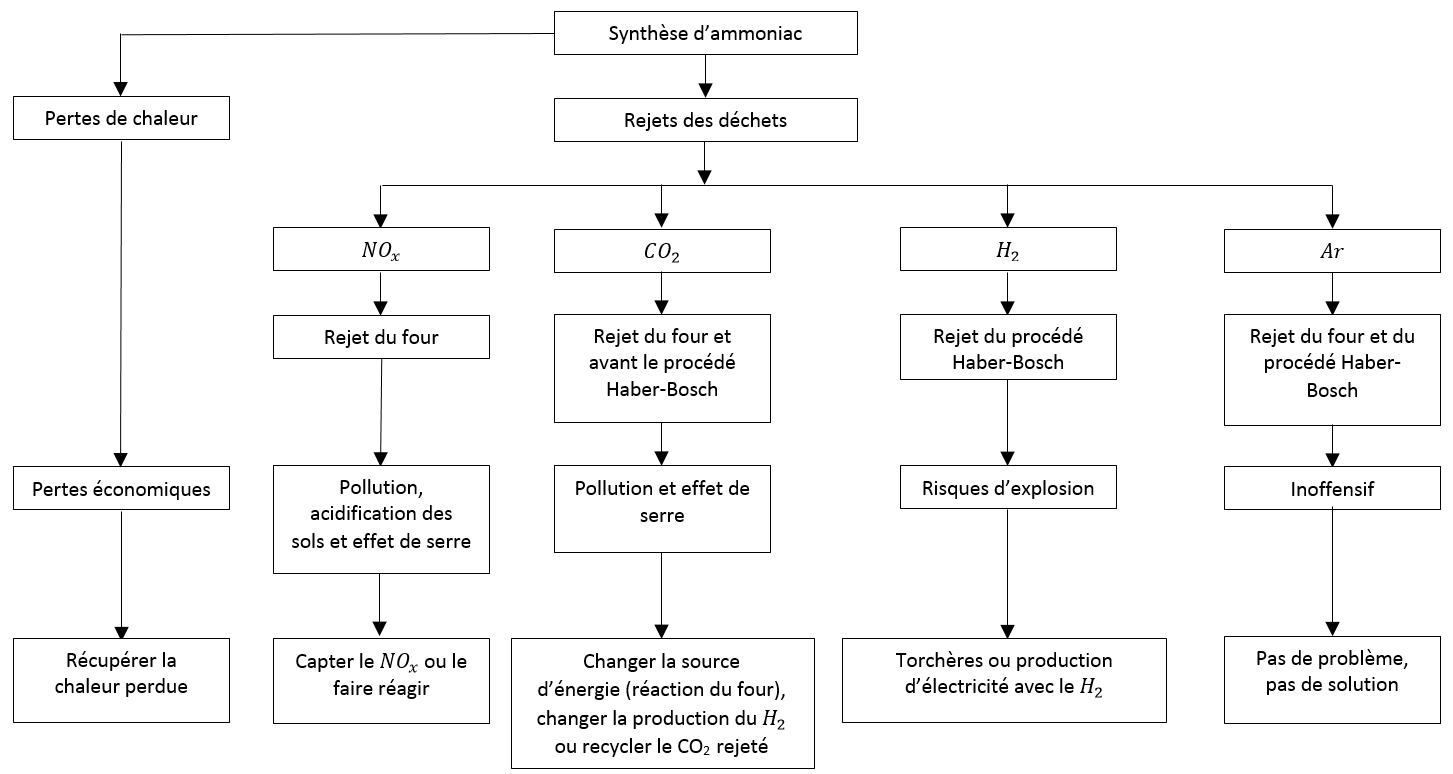
\includegraphics[scale=0.40]{media/mindmap.png}
		\end{figure}
	\end{frame}
	
	\begin{frame}
		\frametitle{Démarche}
		\framesubtitle{Choix d'une source d'impact et pistes d'amélioration} % FIX : s ou pas?
		Notre choix : le \chemform{CO_2}.\\
		Deux possibilités : soit \textbf{réduire les émissions}, soit \textbf{recycler}.
		
		Pour reduire les émissions :
		\begin{itemize}
			\item Changer le procédé de combustion ;
			\item Changer le procédé de création de dihydrogène.
		\end{itemize}
		Pour recycler :
		\begin{itemize}
			\item Produire du carburant à partir d'algues ;
			\item Recycler en matière première ;
			\item Revendre le \chemform{CO_2} à d'autres usines.
		\end{itemize}
	\end{frame}
	
		\begin{frame}
		\frametitle{Démarche}
		\framesubtitle{Choix d'une source d'impact et pistes d'amélioration}
		Notre choix : le \chemform{CO_2}.\\
		Deux possibilités : soit \textbf{réduire les émissions}, soit \textbf{recycler}.
		
		Pour reduire les émissions :
		\begin{itemize}
			\item Changer le procédé de combustion ;
			\item Changer le procédé de création de dihydrogène.
		\end{itemize}
		Pour recycler :
		\begin{itemize}
			\item \textbf{Produire du carburant à partir d'algues} ;
			\item Recycler en matière première ;
			\item Revendre le \chemform{CO_2} à d'autres usines.
		\end{itemize}
	\end{frame}
	
	\begin{frame}
		\frametitle{Notre proposition : l'algocarburant}
		\framesubtitle{Fonctionnement du procédé}
		Fonctionnement général des micro-algues \cite{PrixAlgues} :
		\begin{figure}
			\centering
			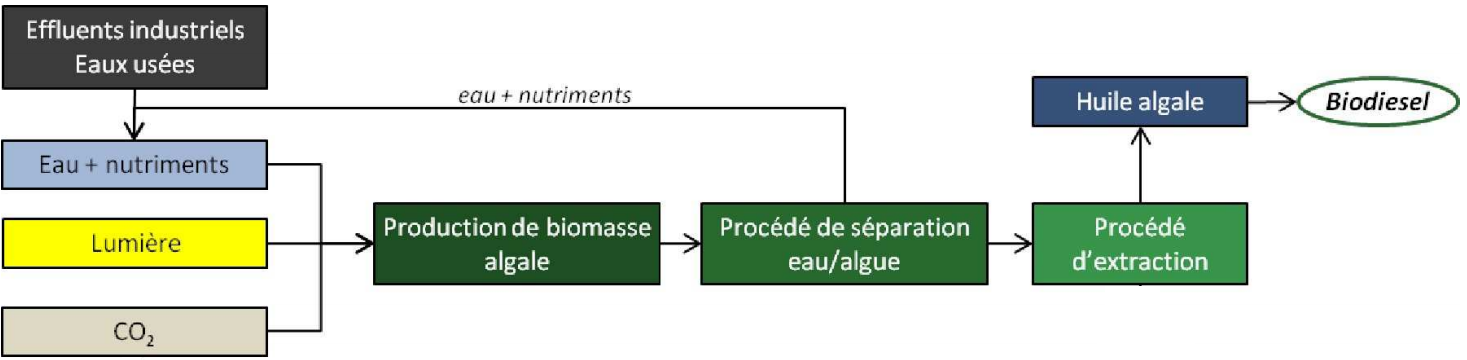
\includegraphics[scale=0.45]{media/fonctionnement-v2.png}
		\end{figure}
	\end{frame}
	
	\begin{frame}
		\frametitle{Notre proposition : l'algocarburant}
		\framesubtitle{Facteurs importants pour le développement des micro-algues}
		\Large{\begin{itemize}
			\item Luminosité (rayons UV) \cite{Lexpansion} ;
			\item Température ;
			\item Régulation des nutriments \cite{BulletinsElec} ;
			\item Qualité du \chemform{CO_2} ;
			\item Types d'algues.
		\end{itemize}}
	\end{frame}
	
	\begin{frame}
		\frametitle{Nos arguments}
		\framesubtitle{Avantages...}
		\begin{center}
			\small{
			\begin{tabular}{p{0.45\textwidth}|p{0.45\textwidth}}
				\textbf{Micro-algues} & \textbf{Algocarburants} \\
				\hline
					\begin{itemize}
						\item[\textcolor{green}{+}] Croissance \cite{BulletinsElec} ;
						\item[\textcolor{green}{+}] Pas de compétition avec les cultures alimentaires ;
						\item[\textcolor{green}{+}] Rendement \cite{Lexpansion}\cite{Enpicbcmed} ;
						\item[\textcolor{green}{+}] Faible empreinte environnementale ;
						\item[\textcolor{green}{+}] Facilité à cultiver \cite{Lexpansion}.
					\end{itemize}   & 
					\begin{itemize}
						\item[\textcolor{green}{+}] Directement consommable par nos moteurs \cite{TPEAlgocarburant} ;
						\item[\textcolor{green}{+}] Rejets de \chemform{CO_2} moins élevés \cite{TPEAlgocarburant}.
					\end{itemize}
			\end{tabular}}
		\end{center}
	\end{frame}
	
	\begin{frame}
		\frametitle{Nos arguments}
		\framesubtitle{... mais aussi quelques inconvénients}
		\begin{itemize}
				\item[\textcolor{red}{-}] Faute de production en masse : prix élevé \cite{Lexpansion} ;
				\item[\textcolor{red}{-}] Extraction de l'huile coûteuse et énergivore \cite{PourLaScience} ;
				\item[\textcolor{red}{-}] Nécessité de rendre le \chemform{CO_2} propre à la 
				consommation des algues ;
				\item[\textcolor{red}{-}] Quantité élevé d'azote et de phosphore
				dans la biomasse \cite{PourLaScience}.
		\end{itemize}
	\end{frame}
	
	\begin{frame}
		\frametitle{Nos arguments}
		\framesubtitle{Etude quantitative}
		Notre production de \chemform{CO_2} : \unit{710 217}{\ton} par an.
		\begin{itemize}
			\item \unit{187 748}{\kilo\gram\per\hectare} de biomasse par an ;
			\item $\rightarrow$ \unit{121 104}{\kilo\gram\per\hectare} d'algocarburant par an \cite{GeneveVillesEtChamps}\cite{TPEMicroalgue} ;
			\item \unit{1}{\kilo\gram} de biomasse fixe \unit{1.8}{\kilo\gram} de \chemform{CO_2}.
		\end{itemize}
		
		\fbox{\begin{minipage}{0.9\textwidth}Avec \unit{246}{\hectare} d'algues, on produit environ \unit{35 084 754}{\liter}
		de carburant par an et on recycle \unit{83134}{\ton} de \chemform{CO_2} par an. C'est à dire 11.7\% 
		de nos émissions.\end{minipage}}
	\end{frame}

	\begin{frame}
		\frametitle{Nos arguments}
		\framesubtitle{D'un point de vue économique}
		\begin{itemize}
			\item Les coûts de production de l'huile varient de 0.5 à 6 euros par tonne ;
			\item Il faut ajouter le coût des différentes étapes
			de raffinage de l'huile ;
			\item Le prix de revient de l'algocarburant est d'environ 5 euros par litre \cite{PrixAlgues}.
		\end{itemize}
		Le prix de vente du baril d'algo-carburant est encore beaucoup trop élevé : \\
		$\rightarrow$ nécessité de continuer le R\&D sur les algocarburants.
	\end{frame}

	%\begin{frame}
		%\section{Conclusion }
		%\frametitle{Plan de l'exposé}
		%\tableofcontents[currentsubsection,sectionstyle=show/shaded,subsectionstyle=show/shaded/hide]
	%\end{frame}
	
	\begin{frame}
	        \section{Bilan de groupe}
		\frametitle{Plan de l'exposé}
		\tableofcontents[currentsubsection,sectionstyle=show/shaded,subsectionstyle=show/shaded/hide]
	\end{frame}
	
	\begin{frame}{Bilan de groupe}
		{\LARGE Point de progrès le plus marquant :}
		
		Amélioration de la régularité du travail en groupe.
		\begin{enumerate}
		\item Réunion de travail hors cours une à plusieurs fois par semaine
		\item Gestion du projet via le site Github
		\end{enumerate}
		\begin{figure}
			\centering
			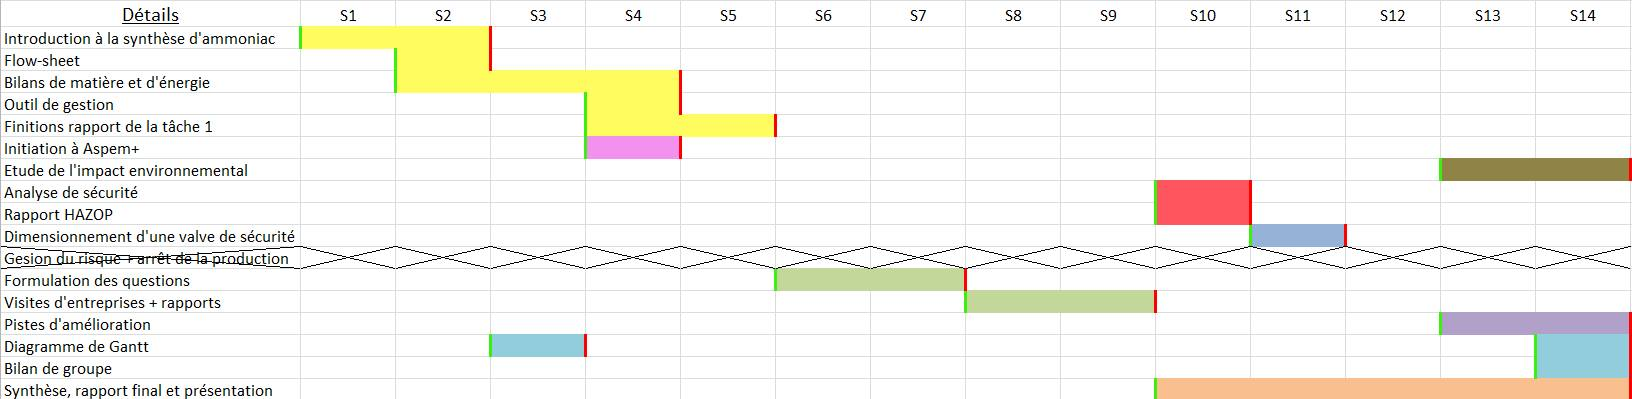
\includegraphics[scale=0.17]{media/DiagrammeDeGantt.png}
		\end{figure}
	\end{frame}
	
	\begin{frame}
		\section{Conclusion}
		\frametitle{Plan de l'exposé}
		\tableofcontents[currentsubsection,sectionstyle=show/shaded,subsectionstyle=show/shaded/hide]
	\end{frame}
	
	\begin{frame}[allowframebreaks]
	\frametitle{Références}
		\tiny
		\bibliographystyle{plain}
		\bibliography{../tache3/sources-tache3,../tache8/sources-tache8}
		\nocite{*}
	\end{frame}
	
\end{document}